\section{Potentials}\label{sec:potential}

The \pot\ classes are the foundation of \galpy\ and were the first part
of the code that we migrated. The approach is the one of
\sectionname~\ref{sec:design-agnostic}: every private compute method
(\texttt{\_evaluate}, \texttt{\_Rforce}, \texttt{\_zforce},
\texttt{\_phitorque}, \texttt{\_dens}, \texttt{\_surfdens}, and the six
second derivatives) resolves the array namespace from its coordinates
and uses it throughout, and the public methods, through the coercion
decorator, bring scalar and \numpy\ inputs onto the namespace of any
backend input. For the majority of \galpy's potentials this was the
whole change, because they are elementary functions of the coordinates.
The remainder use special functions or tabulated quantities: the
basis-function and multipole expansions (\texttt{SCFPotential},
\texttt{MultipoleExpansionPotential}, and their disk variants) use the
associated Legendre and Gegenbauer polynomials; the power-law potential
with an exponential cutoff and the Einasto profile use incomplete gamma
functions; the double-exponential disk uses Bessel functions in a
Hankel-type integral; and the interpolated potentials and the King
profile evaluate splines. These go through the special-function router
and the interpolation layer of \sectionname~\ref{sec:design-numerics}.
All of the potentials, forces, and wrappers in \texttt{galpy.potential}
run on both backends, with the exception of the potentials that read
$N$-body snapshots through \texttt{pynbody} \citep{Pontzen2013} and
the interface \citep{Webb2020} to \texttt{AMUSE}
\citep{PortegiesZwart2009,Pelupessy2013,PortegiesZwart2018}, which
have no backend code. Even the adiabatic-contraction wrapper, whose
construction is a root find for the contracted profile, builds that
profile on the backend when one of its parameters, or a parameter of
one of the potentials that it contracts, is being differentiated. The
convenience functions that act on potentials (the circular velocity
and epicycle frequencies, the radius of a circular orbit of given
angular momentum or energy, the enclosed mass, and the tidal radius
and tidal tensor of \citealt{Webb2019}) are backend-aware as well;
those that require a root are solved with the shared root finder and
those that require an integral use Gauss--Legendre quadrature.

The derivatives of a potential with respect to the coordinates are, of
course, its forces and second derivatives, which \galpy\ implements by
hand. Under a backend, these can also be obtained by differentiating
the potential, and the agreement between the two is a strong test of
both:
for the basis-function expansions, the spiral arms, a rotating bar, and
composite potentials, the force by automatic differentiation agrees
with the hand-coded force
to a few parts in $10^{15}$, within twenty units in the last place
(\figurename~\ref{fig:adforces}), that is, the derivative that
automatic differentiation
produces is the analytic force up to rounding. While the test suite
checks these identities for every potential, under both backends and in
both modes, the derivatives that matter to the user are those with
respect to the parameters: a potential constructed with a backend array
as a parameter is differentiable with respect to that parameter through
every method. For example, the derivative of the radial force of a Miyamoto--Nagai 
potential with respect to its scale length $a$ reads with \jax\ as
\begin{code}
from galpy.potential import MiyamotoNagaiPotential
def Rforce_of_a(a):
    mp= MiyamotoNagaiPotential(amp=1.,a=a,b=0.3)
    return mp.Rforce(1.2,0.1)
dFR_da= jax.grad(Rforce_of_a)(0.5)
\end{code}
and the same with \torch\ is
\begin{code}
a= torch.tensor(0.5,requires_grad=True)
mp= MiyamotoNagaiPotential(amp=1.,a=a,b=0.3)
mp.Rforce(torch.tensor(1.2),
          torch.tensor(0.1)).backward()
a.grad # dFR/da
\end{code}
All 47 potentials that can be constructed from parameters alone are
differentiable with respect to their amplitude (or, for the King
model, its mass) in this way, both eagerly and under
compilation. \figurename~\ref{fig:paramgrad}
displays the accuracy of these parameter derivatives and a small
example of their use, the recovery of the scale length of a Plummer
potential from its force by gradient descent. The parameters of a
potential constructed from a density, as the basis-function and
multipole expansions and their disk variants can be, carry the
derivative through the expansion coefficients.

\begin{figure*}[t!]
  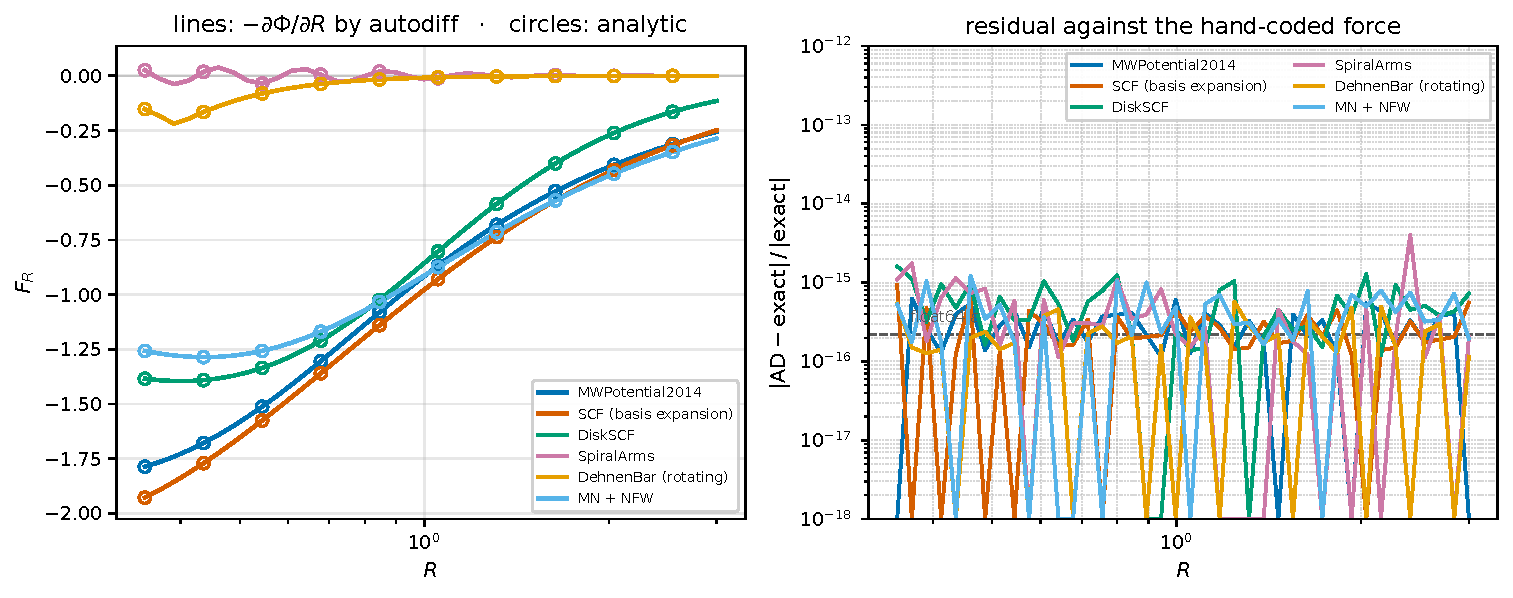
\includegraphics[width=\textwidth,clip=]{../figures/gF1_autodiff_forces/gF1_autodiff_forces.pdf}
  \caption{The radial force by automatic differentiation of the
    potential compared with the hand-coded force, for the Milky-Way
    model, a basis-function expansion and its disk variant, spiral arms,
    a rotating bar, and a disk-plus-halo composite. Left: the force along
    $R$ in the mid-plane, lines from automatic differentiation and
    circles from the analytic implementation. Right: the relative
    difference between the two, which is at the level of the
    double-precision rounding error.}\label{fig:adforces}
\end{figure*}

\begin{figure*}[t!]
  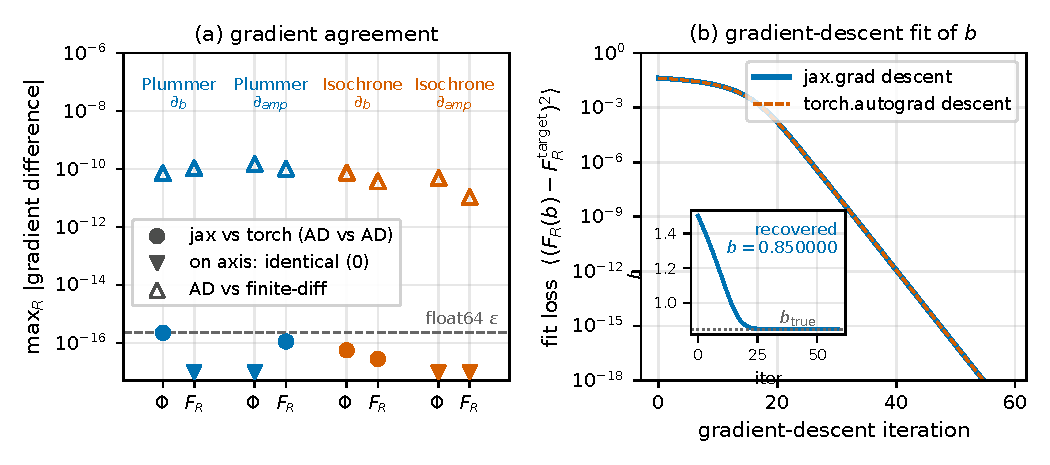
\includegraphics[width=\textwidth,clip=]{../figures/g3_param_gradients/g3_param_gradients.pdf}
  \caption{Derivatives of potentials with respect to their parameters.
    The left panel shows, for the Plummer and isochrone potentials, the
    largest difference between the derivatives of the potential and of
    the radial force with respect to the amplitude and scale parameters
    computed with \jax\ and with \torch\ (circles, at the level of the
    double-precision rounding error; where the two are bit-identical, the
    difference is zero and cannot be shown on the logarithmic axis, which
    the filled triangles on the axis mark) and between either of these and a
    central finite difference (open triangles, at the level of the
    finite-difference error). The right panel displays the recovery of
    the scale length of a Plummer potential from the radial force at a
    set of points by gradient descent on the derivative, starting from
    $b=1.5$ and converging to the true $b=0.85$, with both
    backends.}\label{fig:paramgrad}
\end{figure*}

The backend potentials differ from the \numpy\ ones in a few respects.
Where \galpy\ computes an integral over a potential adaptively on the
\numpy\ path, as for the enclosed mass of a general density or the
surface density, the backend computes a fixed-order Gauss--Legendre
approximation; we set the order such that the two agree, but the backend
result is an approximation of fixed cost rather than an adaptive one. Interpolated potentials evaluate
the same spline as \scipy\ does, to within one unit in the last place,
by converting the fitted spline to a piecewise-polynomial table; they are
differentiable in the evaluation point and, when they are built from a
potential or function with a parameter that is being differentiated,
also in the tabulated values, because the table and the spline
coefficients are then computed on the backend and the derivative with
respect to the parameter passes through them.
A potential that moves along a precomputed orbit, as the
\texttt{MovingObjectPotential}, interpolates that orbit on the backend
when the orbit was integrated there, such that the field of the moving
object is differentiable with respect to everything that the orbit
depends on, and lives on the GPU when the orbit does; an orbit
integrated with \numpy\ stays on \numpy\ and the field is computed at
backend coordinates. And a \python\ branch on the
value of a stored parameter, such as the special case of a vanishing
scale length, is harmless when the parameter is differentiated eagerly
but fails when the parameter is traced inside a compiled ODE solve; we
replaced such branches where we found them, but authors of new
potentials should keep this behavior in mind.

New potentials are written as before: a class that inherits from
\pot\ and implements \texttt{\_evaluate}, \texttt{\_Rforce}, and
\texttt{\_zforce}. If these are written with the resolved namespace
rather than with \numpy\ directly, as illustrated in \figurename~\ref{fig:newpot},
the new potential runs on every backend and can be differentiated with
respect to its parameters without any further work, and the test suite's
automatic checks of new potentials are run under every backend. A test
checks that no migrated potential calls \numpy\ directly in a compute
method.

\begin{figure}[t!]
\begin{codefig}
from galpy.potential import Potential
from galpy.backend import get_namespace
class MNLikePotential(Potential):
    # a Miyamoto-Nagai disk written for every backend
    def __init__(self,amp=1.,a=1.,b=0.1,
                 normalize=False):
        Potential.__init__(self,amp=amp)
        self._a= a
        self._b2= b**2
        if normalize: self.normalize(normalize)
    def _evaluate(self,R,z,phi=0.,t=0.):
        xp= get_namespace(R,z)
        s= self._a+xp.sqrt(z**2+self._b2)
        return -1./xp.sqrt(R**2+s**2)
    def _Rforce(self,R,z,phi=0.,t=0.):
        xp= get_namespace(R,z)
        s= self._a+xp.sqrt(z**2+self._b2)
        return -R*(R**2+s**2)**-1.5
    def _zforce(self,R,z,phi=0.,t=0.):
        xp= get_namespace(R,z)
        sqb= xp.sqrt(z**2+self._b2)
        s= self._a+sqb
        return -z*s/sqb*(R**2+s**2)**-1.5
# differentiate an orbit in it w.r.t. the scale length a
def final_z(a):
    o= Orbit(jnp.asarray([1.,0.1,1.1,0.1,0.05,0.]))
    mp= MNLikePotential(a=a,b=0.3,normalize=1.)
    o.integrate(ts,mp,method='diffrax')
    return o.z(ts[-1])
jax.grad(final_z)(0.5)
\end{codefig}
\caption{A new \pot\ class written for every backend. The only
  difference from a class written for \numpy\ is that the array
  functions are taken from the namespace resolved from the coordinates
  (\texttt{xp}) rather than from \numpy. The class can then be used, and
  differentiated, like any other potential; the last lines take the
  derivative of the final height of an orbit with respect to the scale
  length of the new potential.}\label{fig:newpot}
\end{figure}
